

Even though the total number of tests is growing, it is worth seeing if the mix of tests is changing at all. We have used a $\chi^2$ test to see if the counts of tests yielding different eGFR values is changing over time. The eGFR values have been put into five categories using cut-offs of 15, 30, 60, and 90

\begin{Schunk}
\begin{Soutput}
'data.frame':	195 obs. of  5 variables:
 $ X     : Factor w/ 195 levels "1","10","100",..: 1 108 119 130 141 152 163 174 185 2 ...
 $ Year  : Factor w/ 4 levels "2013","2014",..: 1 1 1 1 1 1 1 1 1 1 ...
 $ Month : Factor w/ 12 levels "1","10","11",..: 1 1 1 1 1 5 5 5 5 5 ...
 $ EGFR_G: Factor w/ 5 levels "(-1,15]","(15,30]",..: 1 2 3 4 5 1 2 3 4 5 ...
 $ n     : num  37 193 1073 2690 1838 ...
\end{Soutput}
\end{Schunk}

The test has a $\chi^2$ value of 3175.89 (p=0, df=152) which means there is a change in the pattern of testing over time for the five categories.

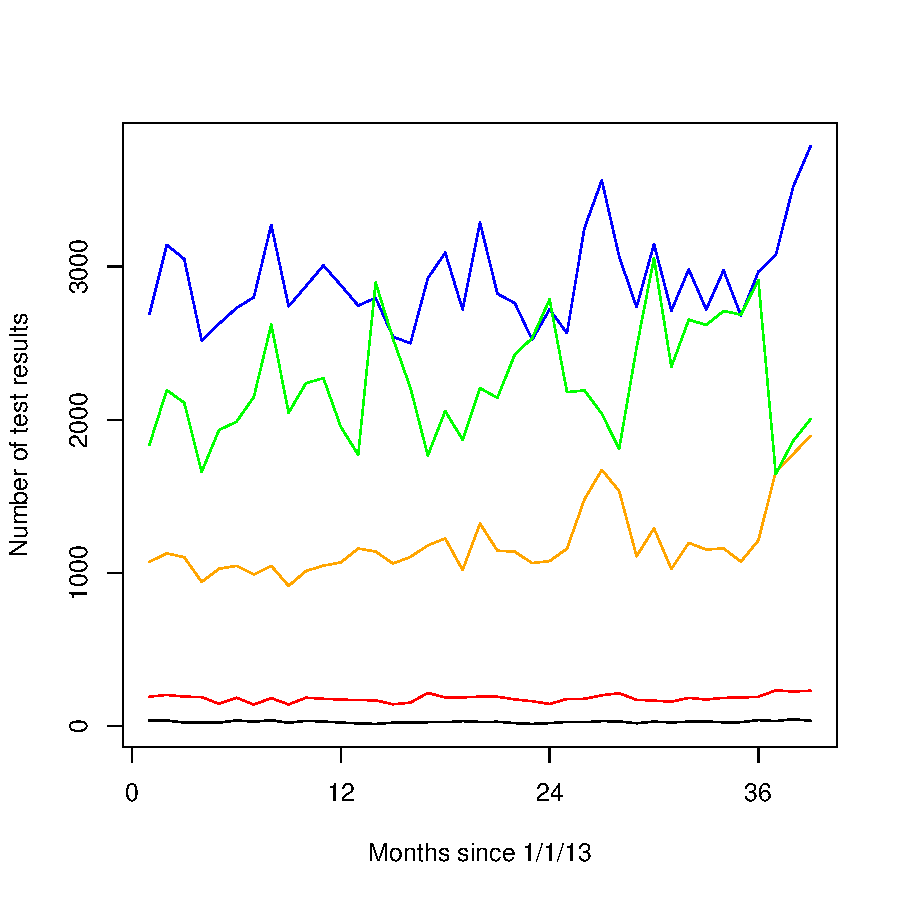
\includegraphics{Figures/Monthly-LinePlots}

It is difficult to see any growth in the number of tests being conducted for patients whose eGFR is between 60 and 90 (shown in blue) and above 90 (shown in green). The patinet groups of greatest interest are those with eGFR between 30 and 60 (shown in orange) and between 15 and 30 (shown in red). The numbers of tests being conducted for patients with eGFR below 15 (shown in black) are extremely low and are probably not worth further analysis given how little they contribute to  the total testing workload. 
